\documentclass{paper}


\usepackage{epsfig}
\usepackage{graphicx}
\usepackage{amsmath}
\usepackage{amssymb}
\usepackage{amsthm}

\usepackage{color}
\usepackage{subcaption}
\usepackage{caption}




\usepackage{mathrsfs}
\usepackage{algpseudocode}
\usepackage{algorithm}

\usepackage{float}
\usepackage{mathtools}
\usepackage{mdwlist}
\usepackage{gensymb}
\usepackage{array}
\usepackage{multirow}
\usepackage[hmargin=3cm]{geometry}
\usepackage{boxedminipage}
\usepackage{enumerate}


\setlength{\parindent}{0pt}
\setlength{\parskip}{18pt}


\usepackage[latin1]{inputenc} 
\usepackage[T1]{fontenc} 

\usepackage{listings} 
\lstset{% 
   language=Matlab, 
   basicstyle=\small\ttfamily, 
} 






\renewcommand{\algorithmicforall}{\textbf{Foreach}}
\newcommand{\init}{\textbf{INIT }}
\newcommand{\pluseq}{\mathrel{+}=}
\newcommand{\asteq}{\mathrel{*}=}
\newcommand{\myto}{\textbf{TO }}
\newcommand*\colvec[3][]{
    \begin{pmatrix}\ifx\relax#1\relax\else#1\\\fi#2\\#3\end{pmatrix}
}
\newcommand{\myparagraph}[1]{\paragraph{#1}\mbox{}\\}
\DeclarePairedDelimiter\ceil{\lceil}{\rceil}
\DeclarePairedDelimiter\floor{\lfloor}{\rfloor}



\title{Computational Photography Assignment 4}



\author{Single Michael\\08-917-445}
% //////////////////////////////////////////////////


\begin{document}



\maketitle


\section{Poisson Solver}
\subsection{Seamless Cloning}

\subsubsection{Map Example}
\begin{figure}[H]
    \centering
    \begin{subfigure}{1.0\textwidth}
        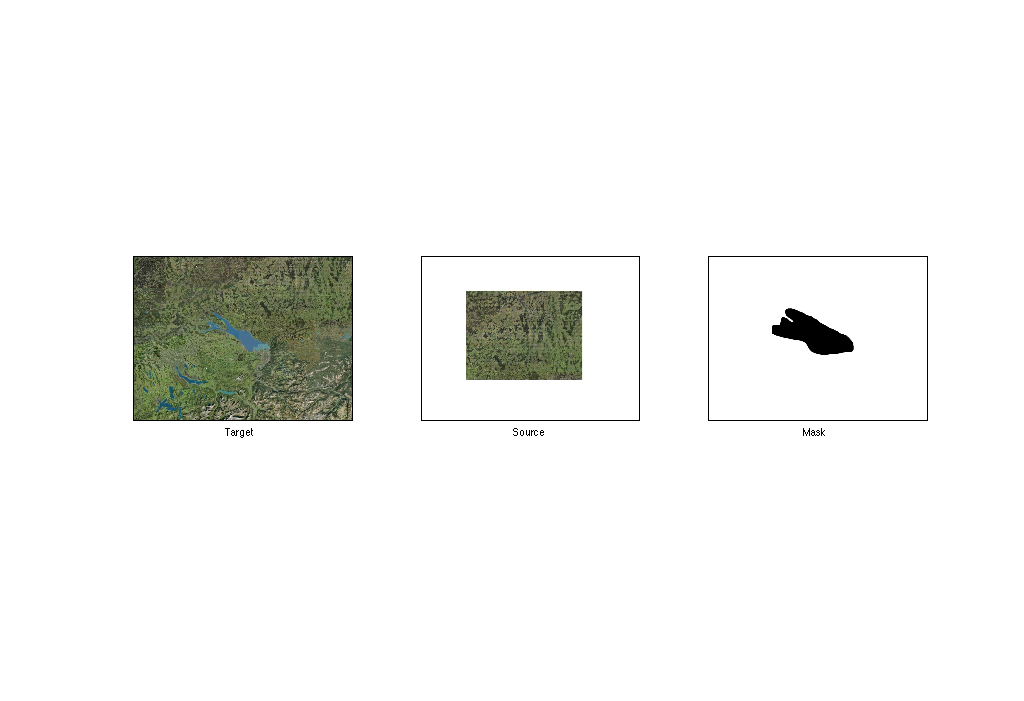
\includegraphics[width=\textwidth]{../../outputs/p4/seamless_cloning/map/input}
    \end{subfigure}
    \caption{Visualization of Input images: Target Image is a texture of a Wall (legt), the source image is a scrible (center), and the corresponding mask (right) having a border of 1, everything else is zero.}
    \label{fig:gradient_mixing_input}       
\end{figure}


\begin{figure}[H]
    \centering
    \begin{subfigure}{1.0\textwidth}
        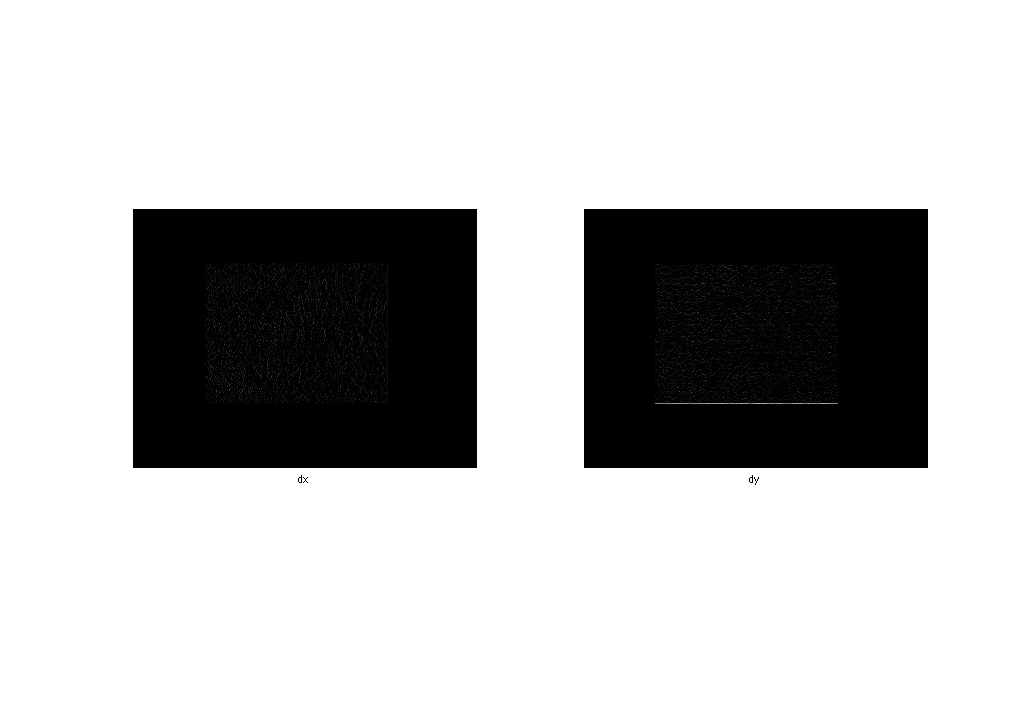
\includegraphics[width=\textwidth]{../../outputs/p4/seamless_cloning/map/gradients}
    \end{subfigure}
    \caption{Visualization of Gradient field along $dx$ and $dy$ resulting from the gradient mixing gradient field applied on each color channel.}
    \label{fig:gradient_mixing_gradients}       
\end{figure}


\begin{figure}[H]
    \centering
    \begin{subfigure}{1.0\textwidth}
        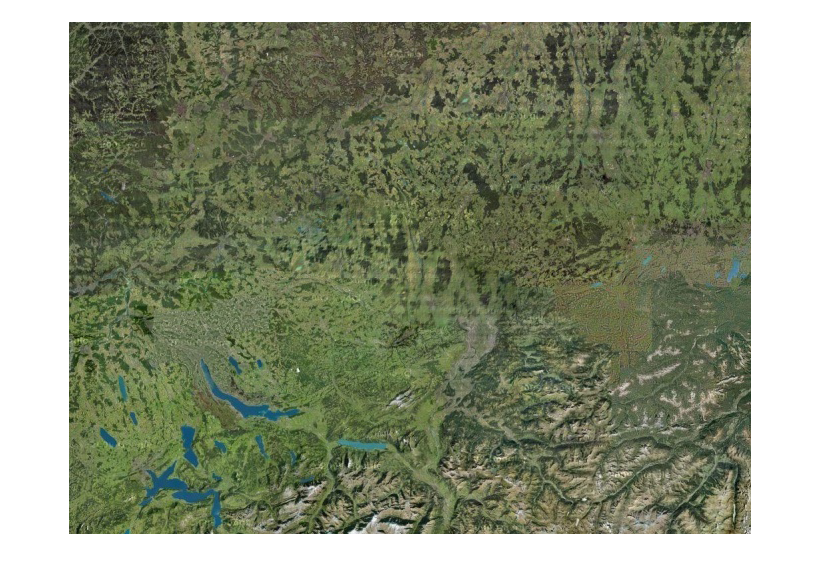
\includegraphics[width=\textwidth]{../../outputs/p4/seamless_cloning/map/output}
    \end{subfigure}
    \caption{Output resulting from the gradient mixing method applied on our given input images using the gradient field as shown above.}
    \label{fig:gradient_mixing_out}       
\end{figure}

\subsubsection{Plane Example}
\begin{figure}[H]
    \centering
    \begin{subfigure}{1.0\textwidth}
        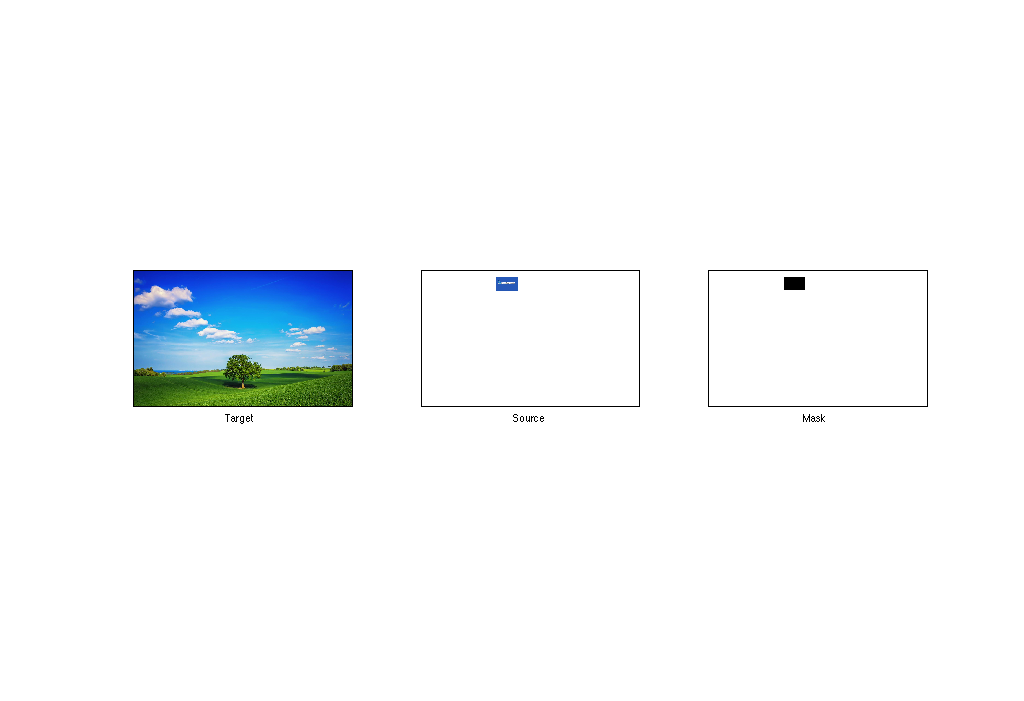
\includegraphics[width=\textwidth]{../../outputs/p4/seamless_cloning/plane/input}
    \end{subfigure}
    \caption{Visualization of Input images: Target Image is a texture of a Wall (legt), the source image is a scrible (center), and the corresponding mask (right) having a border of 1, everything else is zero.}
    \label{fig:gradient_mixing_input}       
\end{figure}


\begin{figure}[H]
    \centering
    \begin{subfigure}{1.0\textwidth}
        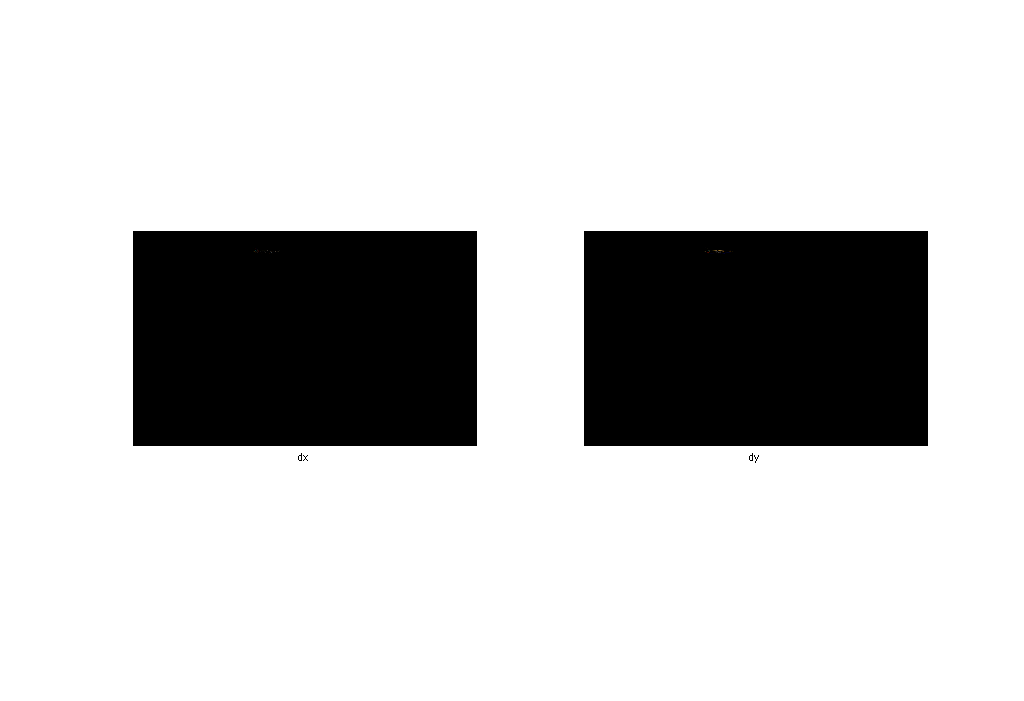
\includegraphics[width=\textwidth]{../../outputs/p4/seamless_cloning/plane/gradients}
    \end{subfigure}
    \caption{Visualization of Gradient field along $dx$ and $dy$ resulting from the gradient mixing gradient field applied on each color channel.}
    \label{fig:gradient_mixing_gradients}       
\end{figure}


\begin{figure}[H]
    \centering
    \begin{subfigure}{1.0\textwidth}
        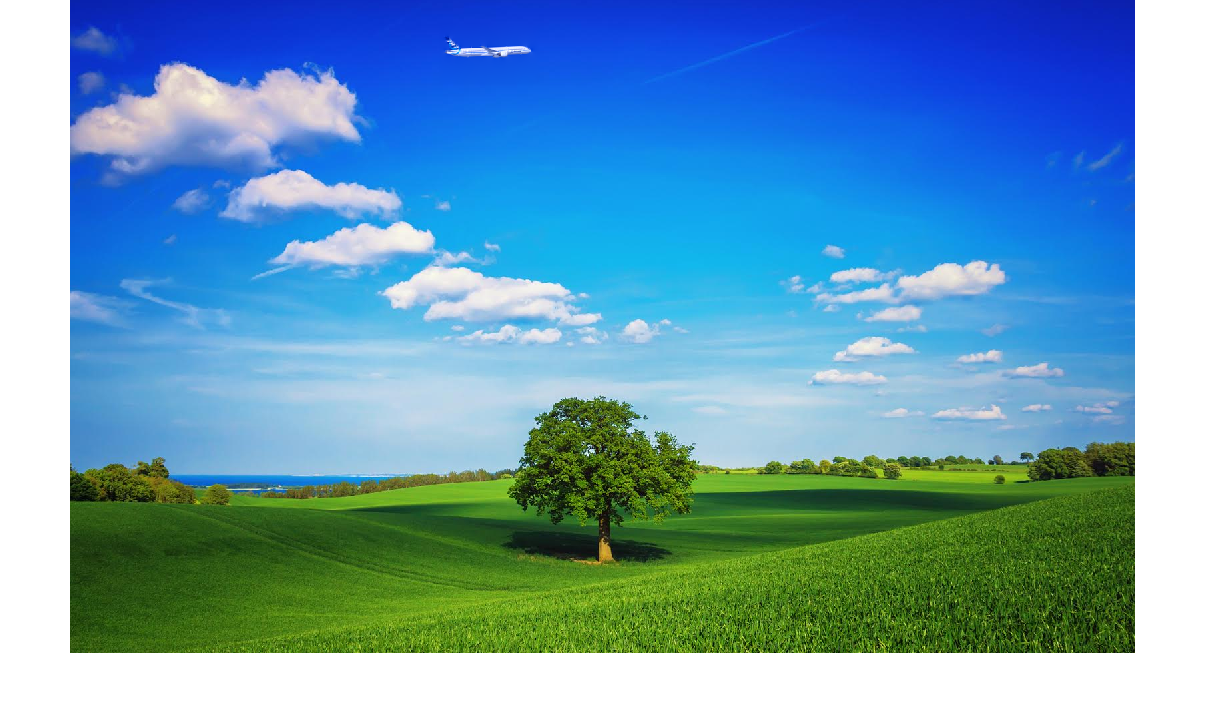
\includegraphics[width=\textwidth]{../../outputs/p4/seamless_cloning/plane/output}
    \end{subfigure}
    \caption{Output resulting from the gradient mixing method applied on our given input images using the gradient field as shown above.}
    \label{fig:gradient_mixing_out}       
\end{figure}

\subsubsection{Monster Example}
\begin{figure}[H]
    \centering
    \begin{subfigure}{1.0\textwidth}
        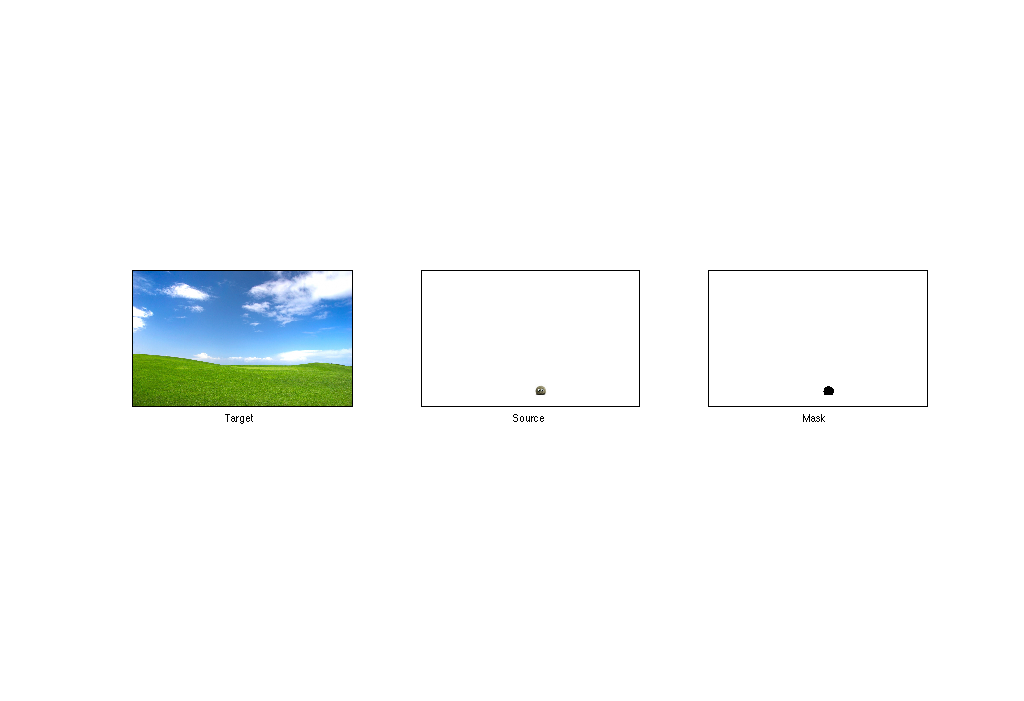
\includegraphics[width=\textwidth]{../../outputs/p4/seamless_cloning/monster/input}
    \end{subfigure}
    \caption{Visualization of Input images: Target Image is a texture of a Wall (legt), the source image is a scrible (center), and the corresponding mask (right) having a border of 1, everything else is zero.}
    \label{fig:gradient_mixing_input}       
\end{figure}


\begin{figure}[H]
    \centering
    \begin{subfigure}{1.0\textwidth}
        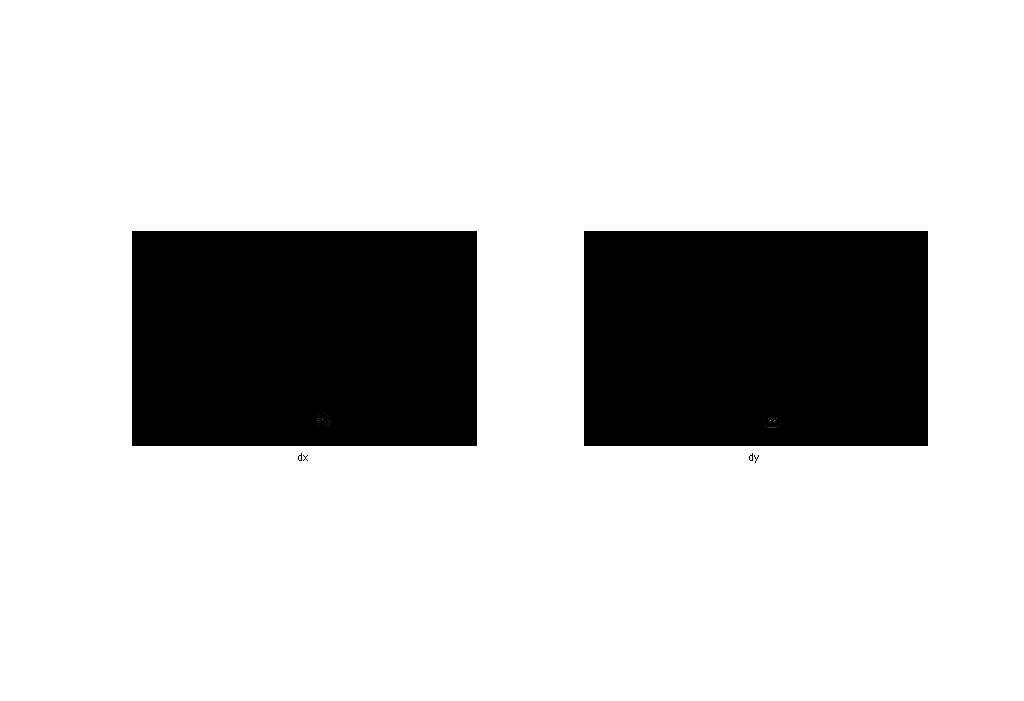
\includegraphics[width=\textwidth]{../../outputs/p4/seamless_cloning/monster/gradients}
    \end{subfigure}
    \caption{Visualization of Gradient field along $dx$ and $dy$ resulting from the gradient mixing gradient field applied on each color channel.}
    \label{fig:gradient_mixing_gradients}       
\end{figure}


\begin{figure}[H]
    \centering
    \begin{subfigure}{1.0\textwidth}
        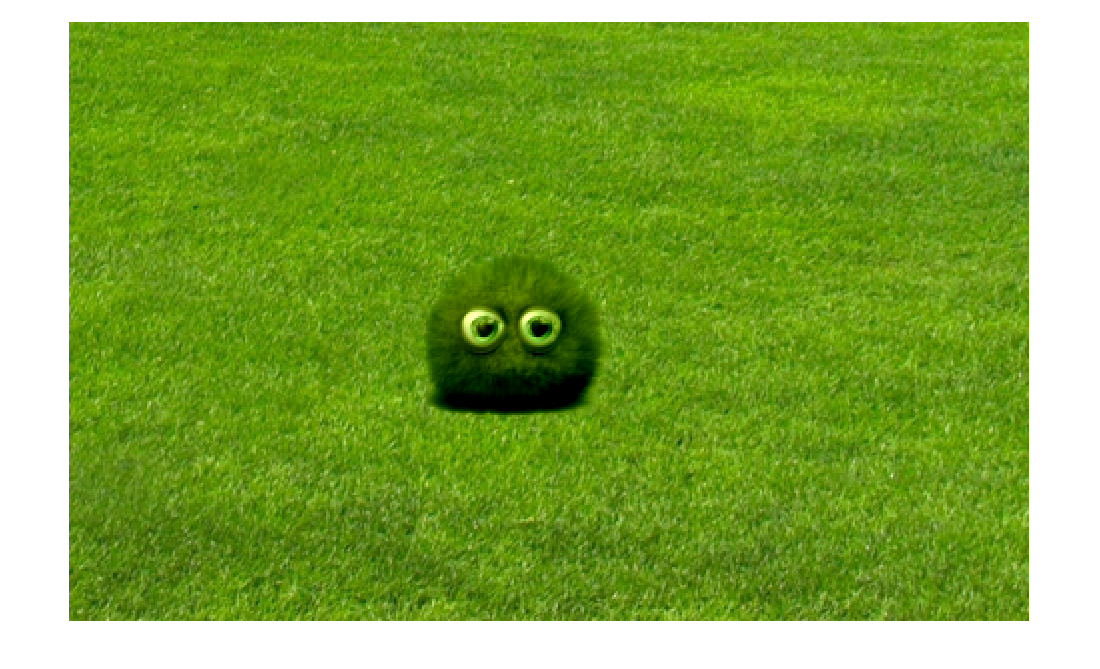
\includegraphics[width=\textwidth]{../../outputs/p4/seamless_cloning/monster/output}
    \end{subfigure}
    \caption{Output resulting from the gradient mixing method applied on our given input images using the gradient field as shown above.}
    \label{fig:gradient_mixing_out}       
\end{figure}



\subsection{Gradient Mixing}

\begin{figure}[H]
    \centering
    \begin{subfigure}{1.0\textwidth}
        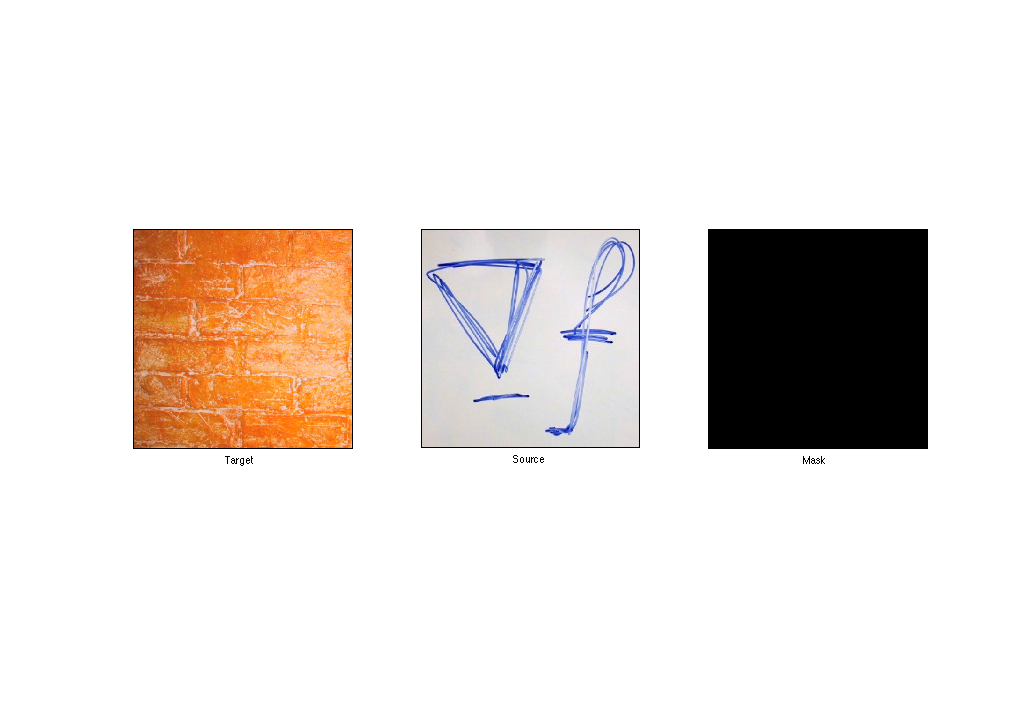
\includegraphics[width=\textwidth]{../../outputs/p4/gradient_mixing/input}
    \end{subfigure}
    \caption{Visualization of Input images: Target Image is a texture of a Wall (legt), the source image is a scrible (center), and the corresponding mask (right) having a border of 1, everything else is zero.}
    \label{fig:gradient_mixing_input}       
\end{figure}


\begin{figure}[H]
    \centering
    \begin{subfigure}{1.0\textwidth}
        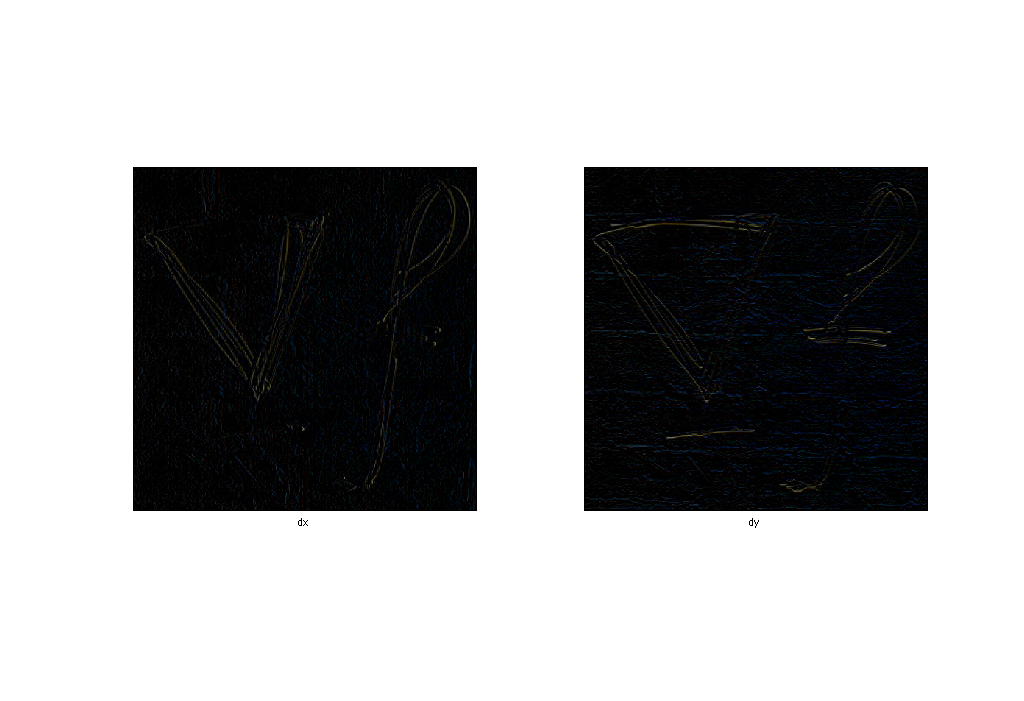
\includegraphics[width=\textwidth]{../../outputs/p4/gradient_mixing/gradients}
    \end{subfigure}
    \caption{Visualization of Gradient field along $dx$ and $dy$ resulting from the gradient mixing gradient field applied on each color channel.}
    \label{fig:gradient_mixing_gradients}       
\end{figure}


\begin{figure}[H]
    \centering
    \begin{subfigure}{1.0\textwidth}
        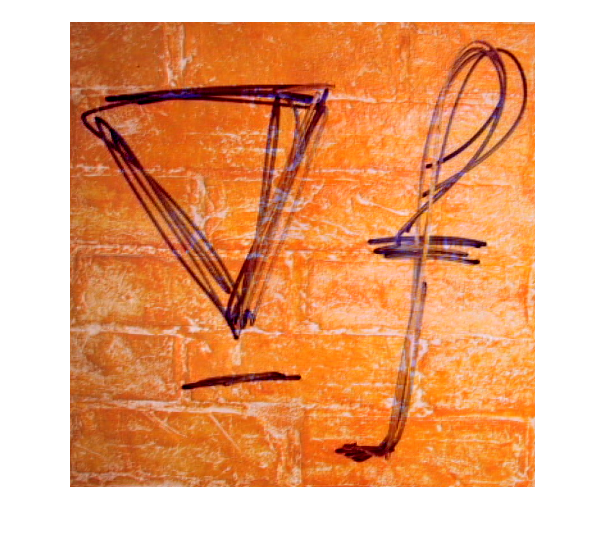
\includegraphics[width=\textwidth]{../../outputs/p4/gradient_mixing/output}
    \end{subfigure}
    \caption{Output resulting from the gradient mixing method applied on our given input images using the gradient field as shown above.}
    \label{fig:gradient_mixing_out}       
\end{figure}

\subsection{Highlight Removal}


\section{Image Segmentation}


\subsection{Sheep Example}

Selection foreground sheep, background grass and some hay in the background gives us quite nice segmentation results.

% input and selection
\begin{figure}[H]
    \centering
    \begin{subfigure}{0.45\textwidth}
        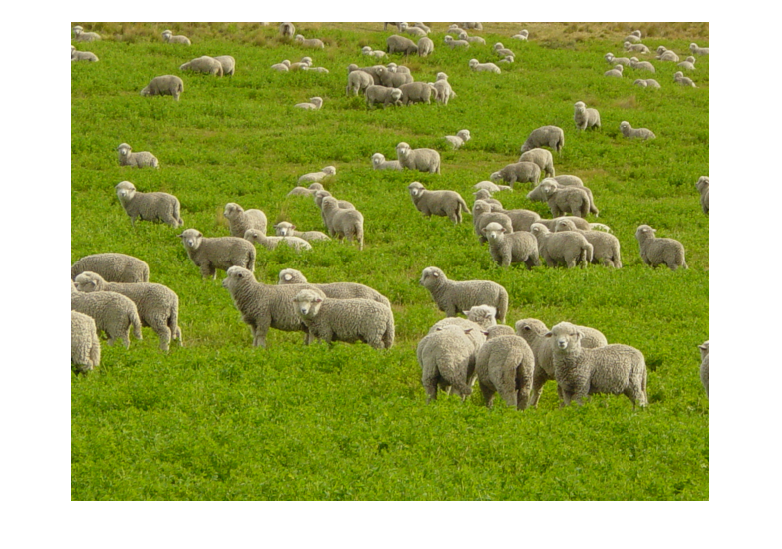
\includegraphics[width=\textwidth]{../../outputs/p4/image_segmentation/sheeps/input}
    \end{subfigure}
    ~
        \begin{subfigure}{0.45\textwidth}
        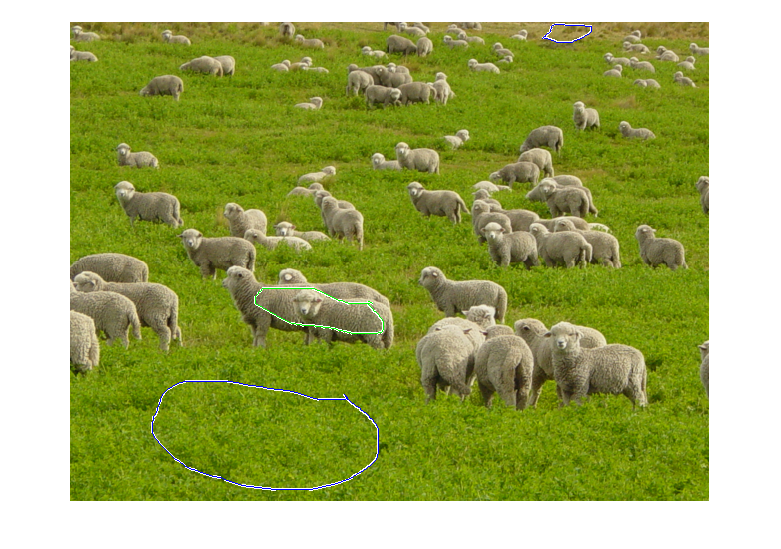
\includegraphics[width=\textwidth]{../../outputs/p4/image_segmentation/sheeps/selection}
    \end{subfigure}
    
    \caption{Used Input (left) and Selection provided by user (right) whereas a green selection indicates foreground and a blue selection indicates the background.}
    \label{fig:segmentation_sheeps_input_selection}       
\end{figure}

% masks
\begin{figure}[H]
    \centering
    \begin{subfigure}{1.0\textwidth}
        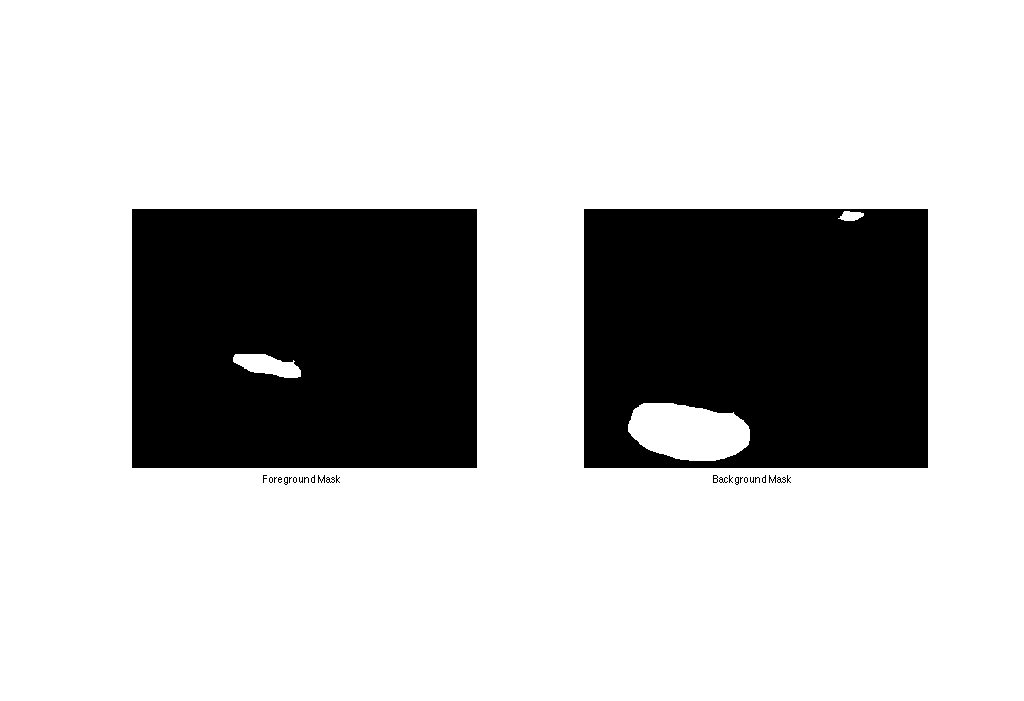
\includegraphics[width=\textwidth]{../../outputs/p4/image_segmentation/sheeps/masks}
    \end{subfigure}
    \caption{On the left the Foreground Mask and on the right the Background mask. For the foreground mask a white regions indicate that such a region should be interpreted as foreground. Similarly for the background mask.}
    \label{fig:segmentation_sheeps_masks}       
\end{figure}


% mean colors
\begin{figure}[H]
    \centering
    \begin{subfigure}{0.45\textwidth}
        
\includegraphics[width=\textwidth]{../../outputs/p4/image_segmentation/sheeps/mean_fg}
    \end{subfigure}
    ~
        \begin{subfigure}{0.45\textwidth}
        
\includegraphics[width=\textwidth]{../../outputs/p4/image_segmentation/sheeps/mean_bg}
    \end{subfigure}
    
    \caption{On the left the foreground mean colors and on the right the mean background colors.}
    \label{fig:segmentation_sheeps_mean_colors}       
\end{figure}


% probabilities
\begin{figure}[H]
    \centering
    \begin{subfigure}{0.45\textwidth}
        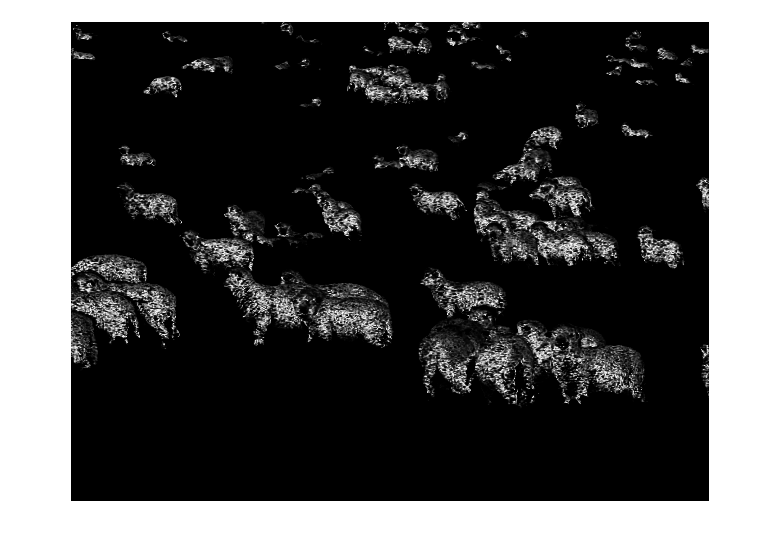
\includegraphics[width=\textwidth]{../../outputs/p4/image_segmentation/sheeps/prob_fg}
    \end{subfigure}
    ~
        \begin{subfigure}{0.45\textwidth}
        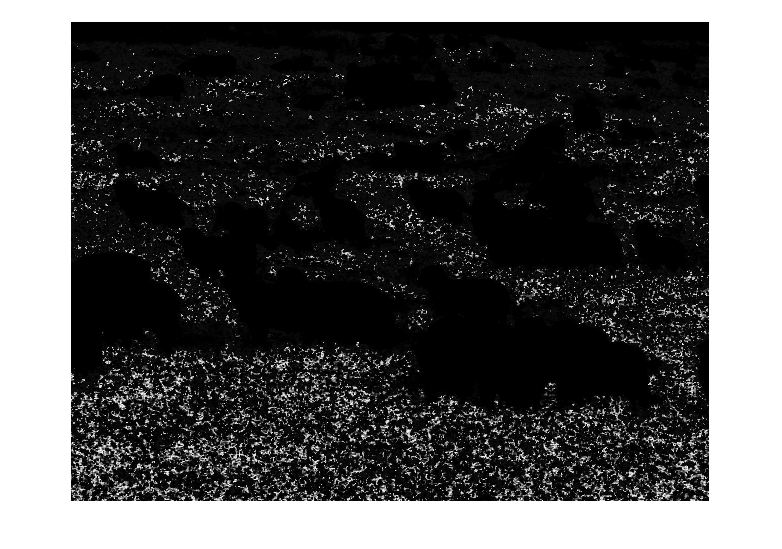
\includegraphics[width=\textwidth]{../../outputs/p4/image_segmentation/sheeps/prob_bg}
    \end{subfigure}
    
    \caption{On the left the probability a pixel belongs to the foreground and on the right the probability a pixel belongs to the background. The whiter the higher the probability is.}
    \label{fig:segmentation_sheeps_probabilities}       
\end{figure}

% smoothness
\begin{figure}[H]
    \centering
    \begin{subfigure}{1.0\textwidth}
        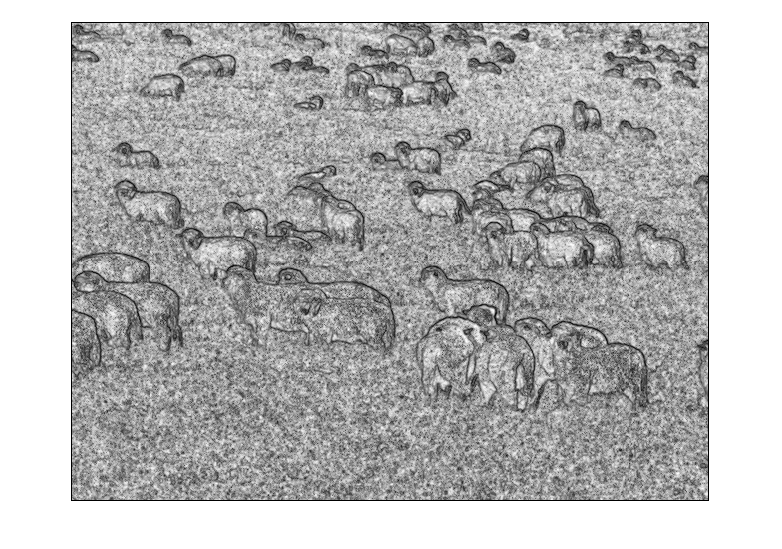
\includegraphics[width=\textwidth]{../../outputs/p4/image_segmentation/sheeps/smoothness}
    \end{subfigure}
    \caption{Illustration of the smoothness term.}
    \label{fig:segmentation_sheeps_smoothness}       
\end{figure}

% segmentation
\begin{figure}[H]
    \centering
    \begin{subfigure}{1.0\textwidth}
        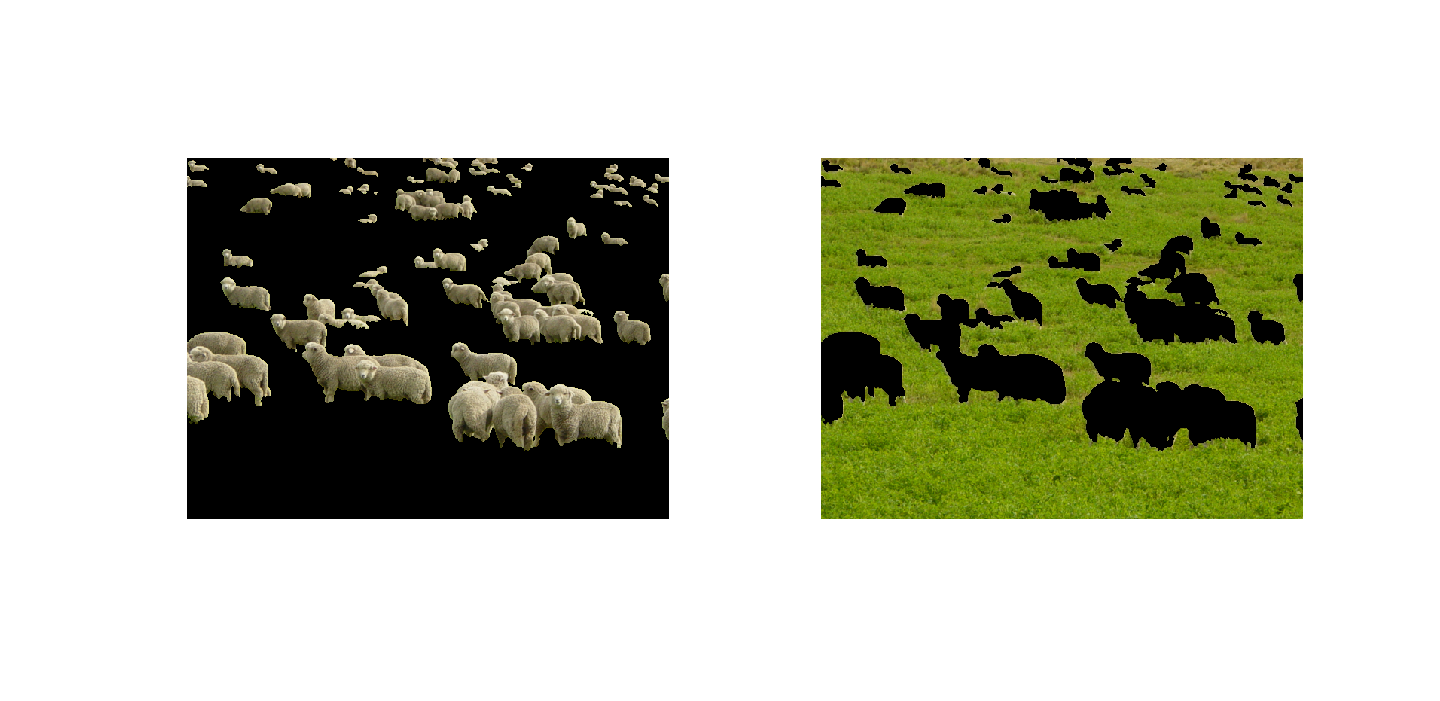
\includegraphics[width=\textwidth]{../../outputs/p4/image_segmentation/sheeps/segmentation}
    \end{subfigure}
    \caption{The segmentation of the image: On the left the Foreground image and on the right the background image}
    \label{fig:segmentation_sheeps_segmenation}       
\end{figure}


\subsection{Zebra Example}

Selection foreground sheep, background grass and some hay in the background gives us quite nice segmentation results.

% input and selection
\begin{figure}[H]
    \centering
    \begin{subfigure}{0.45\textwidth}
        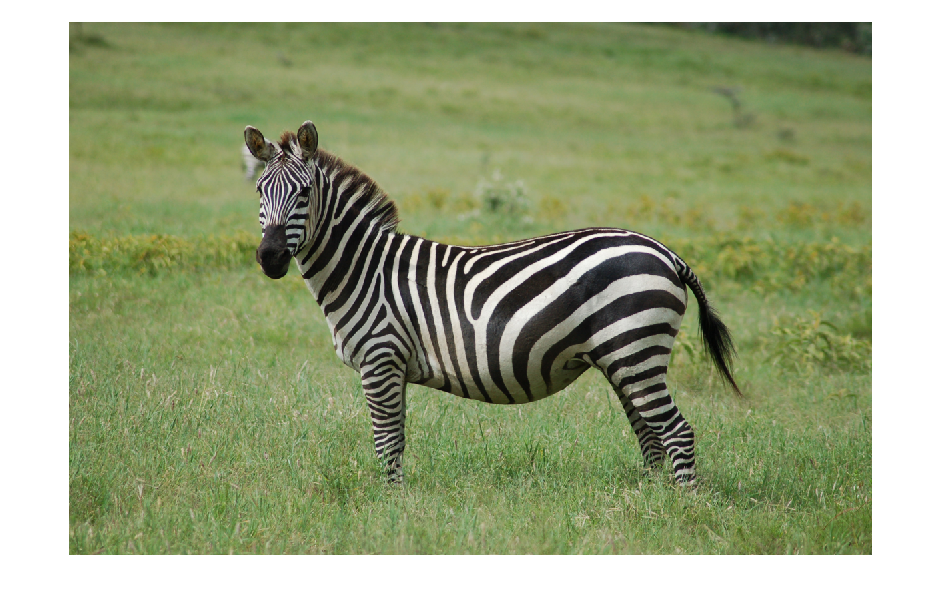
\includegraphics[width=\textwidth]{../../outputs/p4/image_segmentation/zebra/gamma20/input}
    \end{subfigure}
    ~
        \begin{subfigure}{0.45\textwidth}
        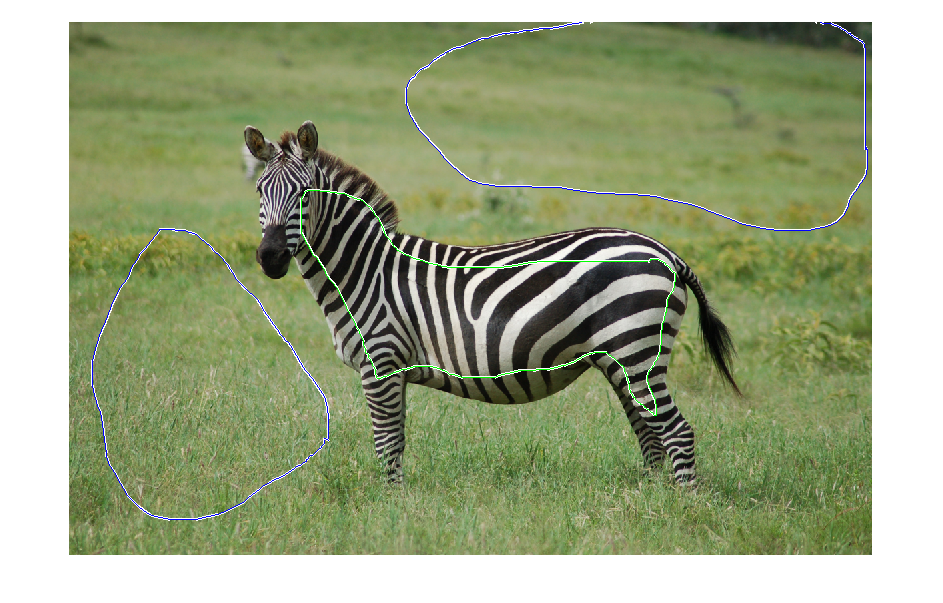
\includegraphics[width=\textwidth]{../../outputs/p4/image_segmentation/zebra/gamma20/selection}
    \end{subfigure}
    
    \caption{Used Input (left) and Selection provided by user (right) whereas a green selection indicates foreground and a blue selection indicates the background.}
    \label{fig:segmentation_zebra_input_selection}       
\end{figure}

% masks
\begin{figure}[H]
    \centering
    \begin{subfigure}{1.0\textwidth}
        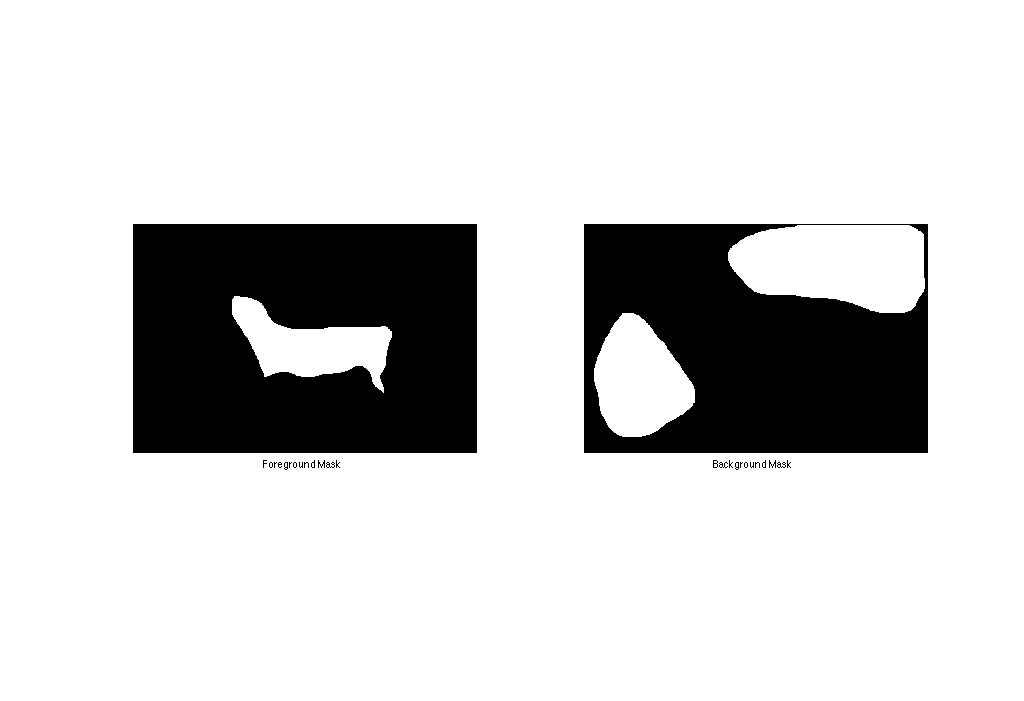
\includegraphics[width=\textwidth]{../../outputs/p4/image_segmentation/zebra/gamma20/masks}
    \end{subfigure}
    \caption{On the left the Foreground Mask and on the right the Background mask. For the foreground mask a white regions indicate that such a region should be interpreted as foreground. Similarly for the background mask.}
    \label{fig:segmentation_zebra_masks}       
\end{figure}


% mean colors
\begin{figure}[H]
    \centering
    \begin{subfigure}{0.45\textwidth}
        
\includegraphics[width=\textwidth]{../../outputs/p4/image_segmentation/zebra/gamma20/mean_fg}
    \end{subfigure}
    ~
        \begin{subfigure}{0.45\textwidth}
        
\includegraphics[width=\textwidth]{../../outputs/p4/image_segmentation/zebra/gamma20/mean_bg}
    \end{subfigure}
    
    \caption{On the left the foreground mean colors and on the right the mean background colors.}
    \label{fig:segmentation_zebra_mean_colors}       
\end{figure}


% probabilities
\begin{figure}[H]
    \centering
    \begin{subfigure}{0.45\textwidth}
        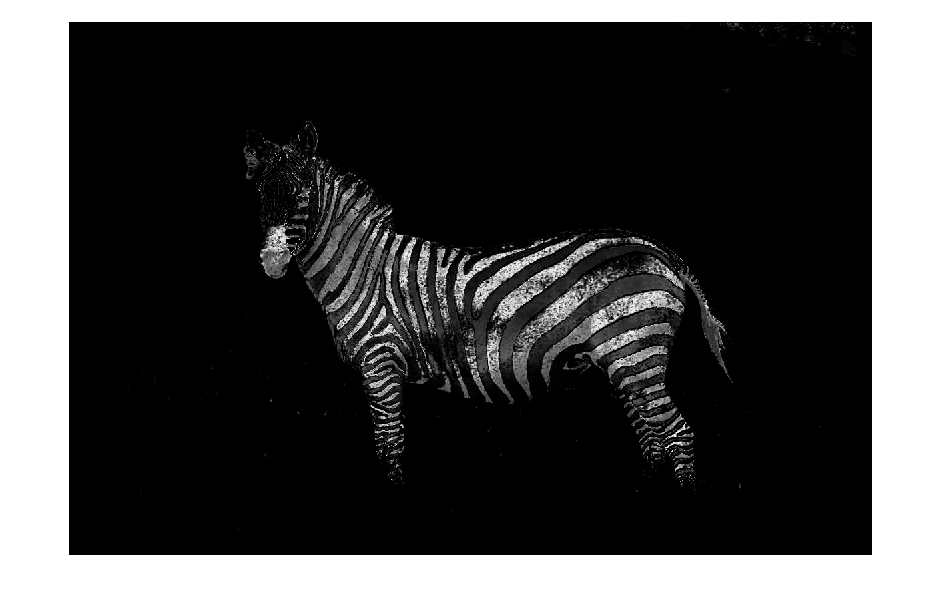
\includegraphics[width=\textwidth]{../../outputs/p4/image_segmentation/zebra/gamma20/prob_fg}
    \end{subfigure}
    ~
        \begin{subfigure}{0.45\textwidth}
        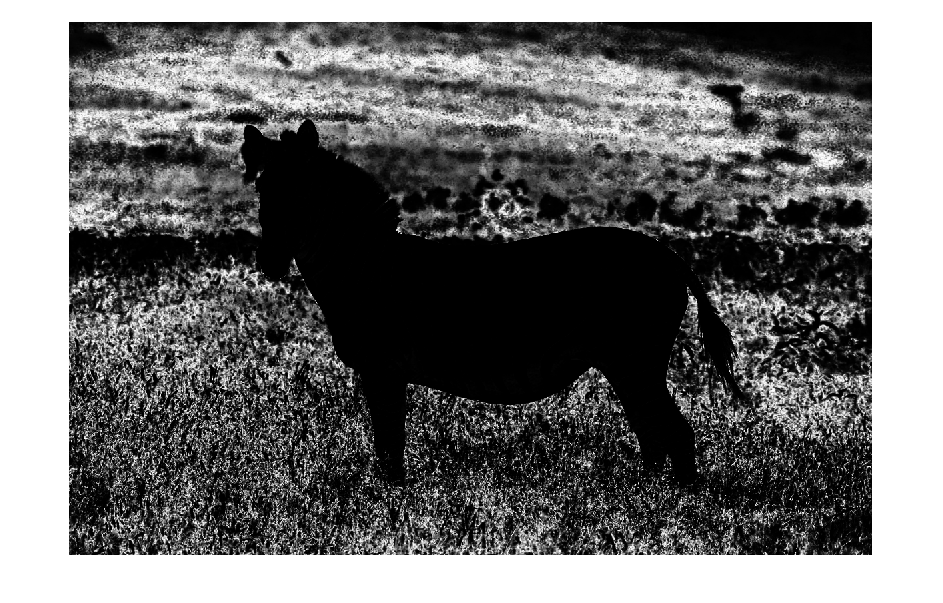
\includegraphics[width=\textwidth]{../../outputs/p4/image_segmentation/zebra/gamma20/prob_bg}
    \end{subfigure}
    
    \caption{On the left the probability a pixel belongs to the foreground and on the right the probability a pixel belongs to the background. The whiter the higher the probability is.}
    \label{fig:segmentation_zebra_probabilities}       
\end{figure}

% smoothness
\begin{figure}[H]
    \centering
    \begin{subfigure}{1.0\textwidth}
        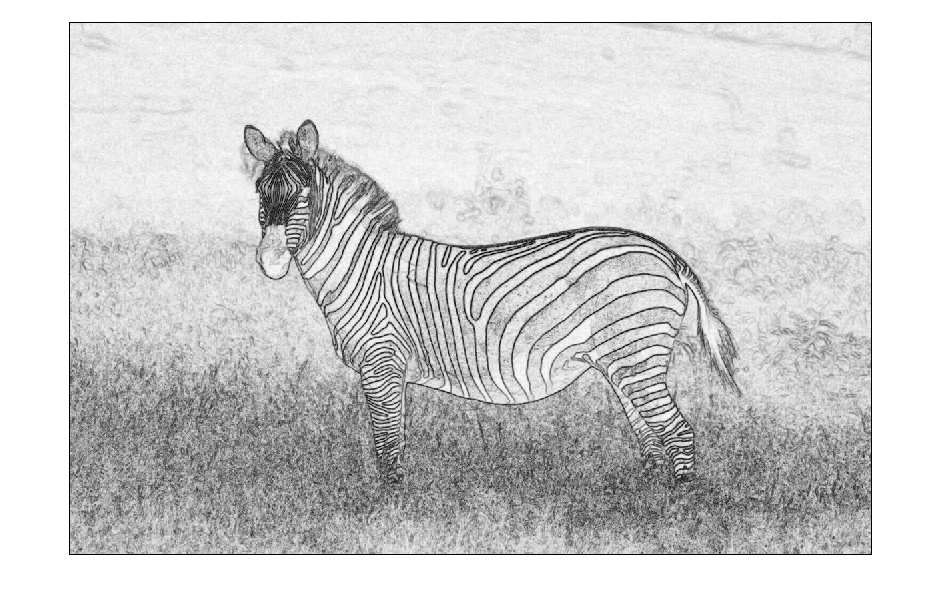
\includegraphics[width=\textwidth]{../../outputs/p4/image_segmentation/zebra/gamma20/smoothness}
    \end{subfigure}
    \caption{Illustration of the smoothness term.}
    \label{fig:segmentation_zebra_smoothness}       
\end{figure}

% segmentation
\begin{figure}[H]
    \centering
    \begin{subfigure}{1.0\textwidth}
        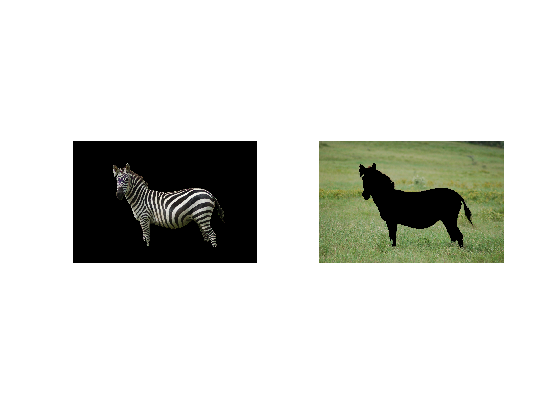
\includegraphics[width=\textwidth]{../../outputs/p4/image_segmentation/zebra/gamma20/segmentation}
    \end{subfigure}
    \caption{The segmentation of the image: On the left the Foreground image and on the right the background image}
    \label{fig:segmentation_zebra_segmenation}       
\end{figure}


\subsection{Second Zebra Example}

Selection foreground sheep, background grass and some hay in the background gives us quite nice segmentation results.

% input and selection
\begin{figure}[H]
    \centering
    \begin{subfigure}{0.45\textwidth}
        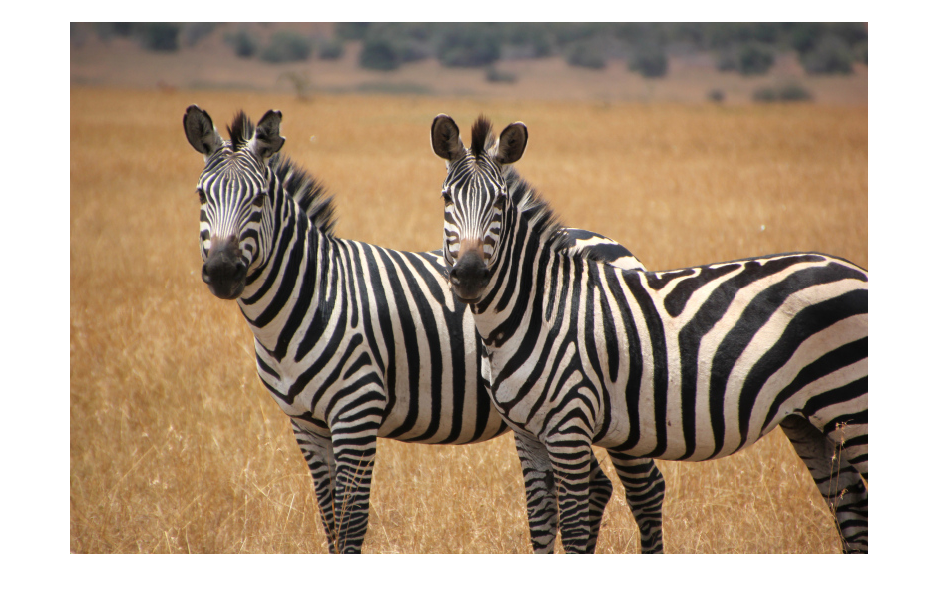
\includegraphics[width=\textwidth]{../../outputs/p4/image_segmentation/zebra2/input}
    \end{subfigure}
    ~
        \begin{subfigure}{0.45\textwidth}
        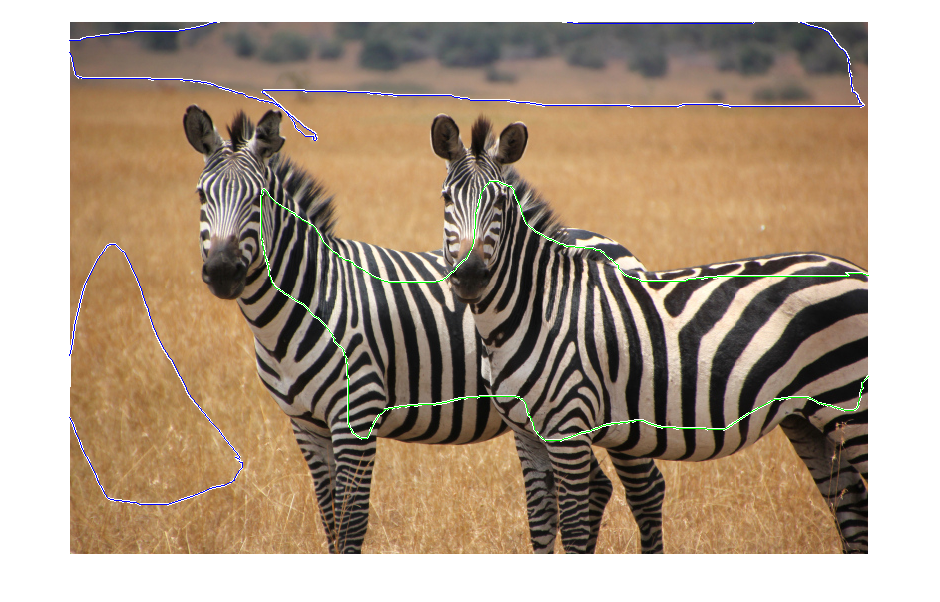
\includegraphics[width=\textwidth]{../../outputs/p4/image_segmentation/zebra2/selection}
    \end{subfigure}
    
    \caption{Used Input (left) and Selection provided by user (right) whereas a green selection indicates foreground and a blue selection indicates the background.}
    \label{fig:segmentation_zebra2_input_selection}       
\end{figure}

% masks
\begin{figure}[H]
    \centering
    \begin{subfigure}{1.0\textwidth}
        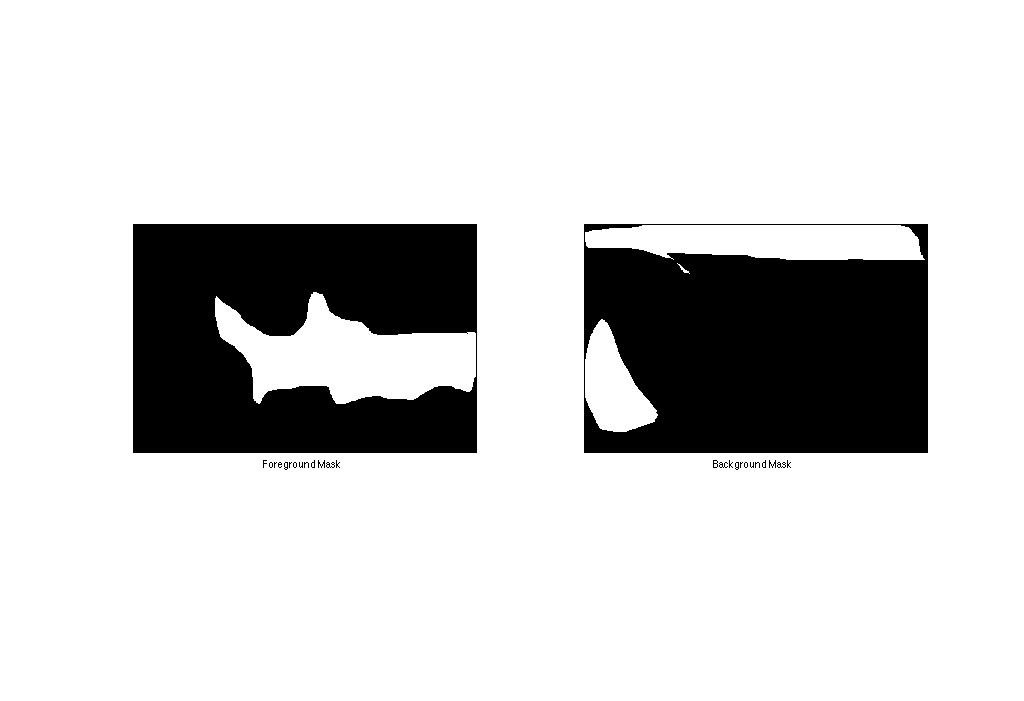
\includegraphics[width=\textwidth]{../../outputs/p4/image_segmentation/zebra2/masks}
    \end{subfigure}
    \caption{On the left the Foreground Mask and on the right the Background mask. For the foreground mask a white regions indicate that such a region should be interpreted as foreground. Similarly for the background mask.}
    \label{fig:segmentation_zebra2_masks}       
\end{figure}


% mean colors
\begin{figure}[H]
    \centering
    \begin{subfigure}{0.45\textwidth}
        
\includegraphics[width=\textwidth]{../../outputs/p4/image_segmentation/zebra2/mean_fg}
    \end{subfigure}
    ~
        \begin{subfigure}{0.45\textwidth}
        
\includegraphics[width=\textwidth]{../../outputs/p4/image_segmentation/zebra2/mean_bg}
    \end{subfigure}
    
    \caption{On the left the foreground mean colors and on the right the mean background colors.}
    \label{fig:segmentation_zebra2_mean_colors}       
\end{figure}


% probabilities
\begin{figure}[H]
    \centering
    \begin{subfigure}{0.45\textwidth}
        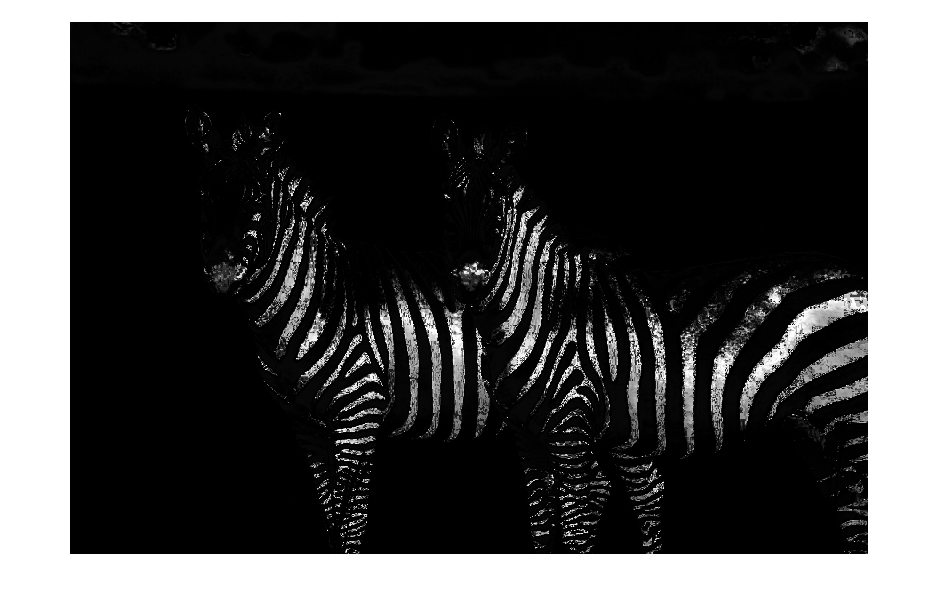
\includegraphics[width=\textwidth]{../../outputs/p4/image_segmentation/zebra2/prob_fg}
    \end{subfigure}
    ~
        \begin{subfigure}{0.45\textwidth}
        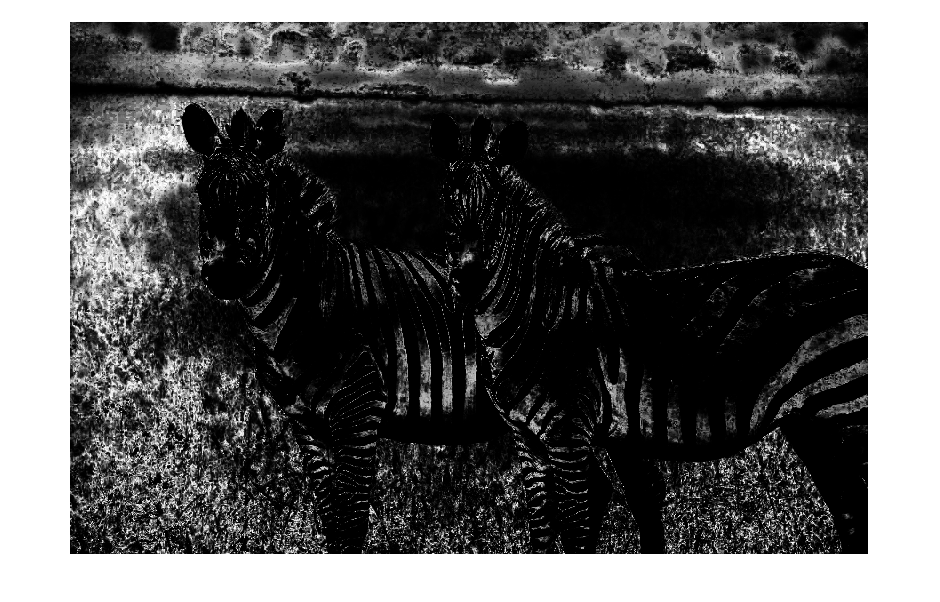
\includegraphics[width=\textwidth]{../../outputs/p4/image_segmentation/zebra2/prob_bg}
    \end{subfigure}
    
    \caption{On the left the probability a pixel belongs to the foreground and on the right the probability a pixel belongs to the background. The whiter the higher the probability is.}
    \label{fig:segmentation_zebra2_probabilities}       
\end{figure}

% smoothness
\begin{figure}[H]
    \centering
    \begin{subfigure}{1.0\textwidth}
        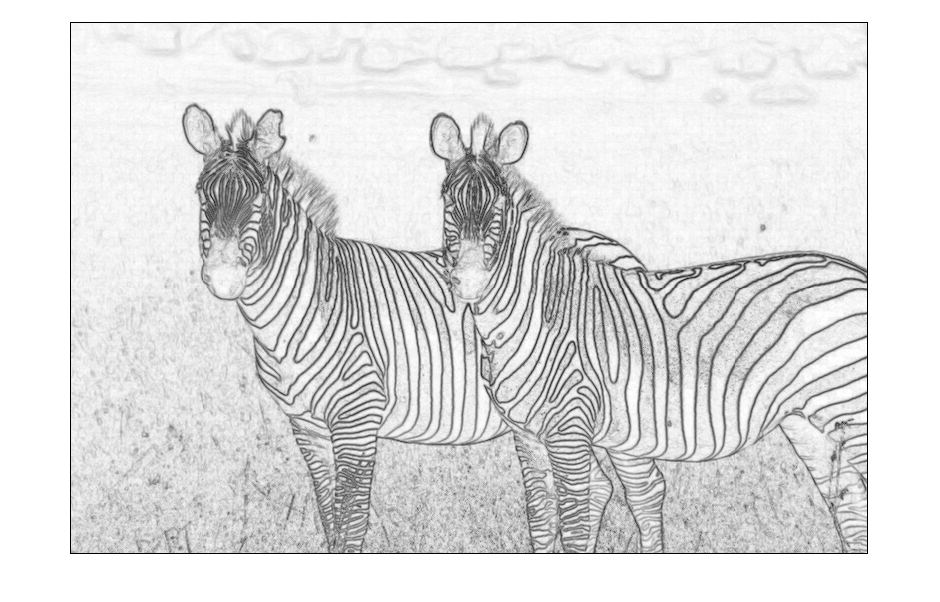
\includegraphics[width=\textwidth]{../../outputs/p4/image_segmentation/zebra2/smoothness}
    \end{subfigure}
    \caption{Illustration of the smoothness term.}
    \label{fig:segmentation_zebra2_smoothness}       
\end{figure}

% segmentation
\begin{figure}[H]
    \centering
    \begin{subfigure}{1.0\textwidth}
        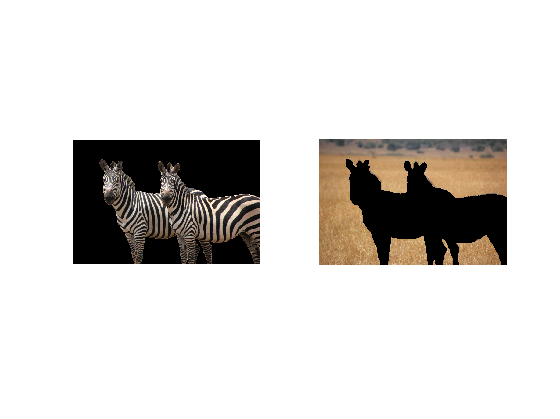
\includegraphics[width=\textwidth]{../../outputs/p4/image_segmentation/zebra2/segmentation}
    \end{subfigure}
    \caption{The segmentation of the image: On the left the Foreground image and on the right the background image}
    \label{fig:segmentation_zebra2_segmenation}       
\end{figure}



\end{document}